\documentclass{cmc}

\begin{document}

\pagestyle{fancy}
\lhead{\textit{\textbf{Computational Motor Control, Spring 2020} \\
    Python exercise, Lab 6, GRADED}} \rhead{Zhou Xiao \\ Lu Xiaolong \\ Joseph Al Aaraj}

\section*{Student names: Zhou Xiao, Lu Xiaolong, Joseph Al Aaraj}
\textit{Instructions: Update this file (or recreate a similar one,
  e.g.\ in Word) to prepare your answers to the questions. Feel free
  to add text, equations and figures as needed. Hand-written notes,
  e.g.\ for the development of equations, can also be included e.g.\
  as pictures (from your cell phone or from a scanner).
  \textbf{\corr{This lab is graded.}} and must be submitted before the
  \textbf{\corr{Deadline : 22-04-2020 23:59}}.  \\ Please submit both
  the source file (*.doc/*.tex) and a pdf of your document, as well as
  all the used and updated Python functions in a single zipped file
  called \corr{lab6\_name1\_name2\_name3.zip} where name\# are the
  team member’s last names.  \corr{Please submit only one report per
    team!}}
\\

\textit{The file \fileref{lab\#.py} is provided to run all exercises
  in Python.
  % Each \fileref{exercise\#.py} can be run to run an exercise
  % individually.
  The list of exercises and their dependencies are shown in
  Figure~\ref{fig:files}.  When a file is run, message logs will be
  printed to indicate information such as what is currently being run
  and and what is left to be implemented. All warning messages are
  only present to guide you in the implementation, and can be deleted
  whenever the corresponding code has been implemented correctly.}


% \textit{In this exercise, you will explore the different modeling
% techniques that can be used to control a single joint and
% segment. We initially start by exploring a single joint controlled
% by a pair of antagonist spring like muscles and then extend the
% model by adding dampers to it. These only represent the passive
% dynamics observed in a real musculoskeletal system. To make the
% behavior more realistic we then study more complex hill muscle model
% in detail. }

\begin{figure}[ht]
  \centering 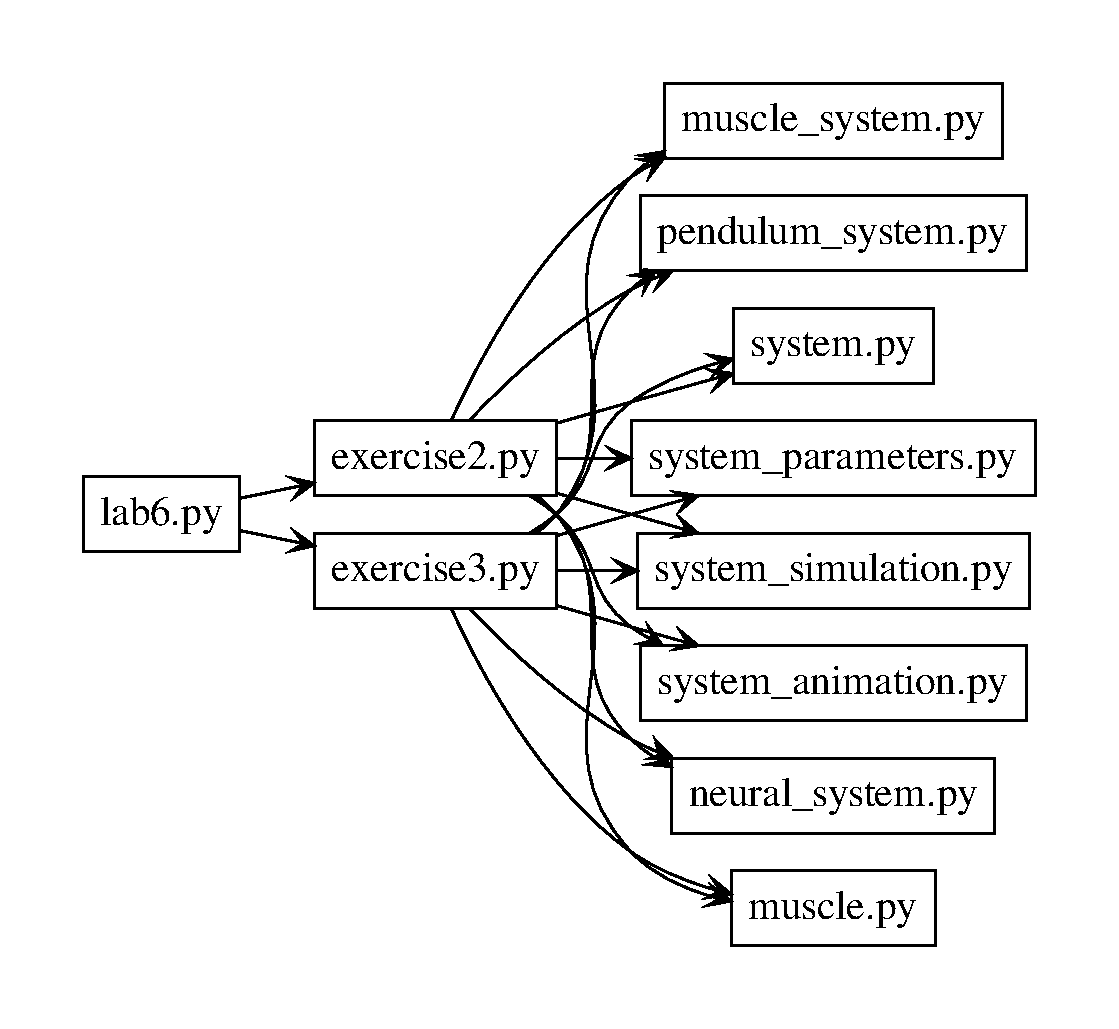
\includegraphics[width=0.5\textwidth]{figures/files}
  \caption{\label{fig:files} Exercise files dependencies. In this lab,
    you will be modifying \fileref{exercise2.py}, \fileref{exercise3.py}
    and optionally \fileref{pendulum\_system.py}}
\end{figure}

\subsection*{Files to complete the exercises}
\label{sec:intro}

\begin{itemize}
\item \fileref{lab6.py} : Main file
\item \fileref{exercise2.py} : Main file to complete exercise 2
\item \fileref{exercise3.py} : Main file to complete exercise 3
\item \fileref{system\_parameters.py} : Parameter class for Pendulum,
  Muscles and Neural Network (Create an instance and change properties
  using the instance. You do not have to modify the file)
\item \fileref{muscle.py} : Muscle class (You do not have to modify
  the file)
\item \fileref{system.py} : System class to combine different models %
  like Pendulum, Muscles, Neural Network (You do not have to modify
  the file)
\item \fileref{pendulum\_system.py} : Contains the description of
  pendulum equation and Pendulum class. You can use the file to define
  perturbations in the pendulum.
\item \fileref{muscle\_system.py} : Class to combine two muscles (You
  do not have to modify the file)
\item \fileref{neural\_system.py} : Class to describe the neural
  network (You do not have to modify the file)
\item \fileref{system\_simulation.py} : Class to initialize all the
  systems, validate and to perform integration (You do not have to
  modify the file)
\item \fileref{system\_animation.py} : Class to produce animation of
  the systems after integration (You do not have to modify the file)
\end{itemize}

\textbf{NOTE : } '\textit{You do not have to modify}' does not mean
you should not, it means it is not necessary to complete the
exercises. But, \corr{you are expected to look into each of these
  files and understand how everything works}. You are free to explore
and change any file if you feel so.

\section*{Exercise 2 : Pendulum model with Muscles}
\label{sec:question-1}

\begin{figure}[H]
  \centering 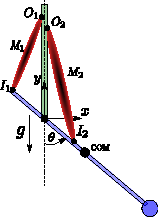
\includegraphics[scale=2.0]{figures/pendulum_muscles.pdf}
  \caption{Pendulum with Antagonist Hill Muscles}
  \label{fig:p_muscles}
\end{figure}

The system is comprised of a physical pendulum described by equation
\ref{eq:pendulum} and a pair of antagonist muscles \textbf{M1} and
\textbf{M2}. Muscle \textbf{M1} extends the pendulum ($\theta$
increases) and Muscle \textbf{M2} flexes the muscle ($\theta$
decreases).

Consider the system only for the pendulum range $\theta$ = $[0, \pi]$

\begin{equation}
  \label{eq:pendulum}
  I\ddot{\theta} = -0.5 \cdot m \cdot g \cdot L \cdot sin(\theta)
\end{equation}

Where,

\begin{itemize}
\item $I$ - Pendulum inertia about the pendulum pivot joint
  [$kg \cdot m^2$]
\item $\theta$ - Pendulum angular position with the vertical [$rad$]
\item $\ddot{\theta}$ - Pendulum angular acceleration
  [$rad \cdot s^{-2}$]
\item $m$ - Pendulum mass [$kg$]
\item $g$ - System gravity [$m \cdot s^{-2}$]
\item $L$ - Length of the pendulum [$m$]
\end{itemize}

Each muscle is modelled using the Hill-type equations that you are now
familiar with.  Muscles have two attachment points, one at the origin
and the other at the insertion point.  The origin points are denoted
by $O_{1,2}$ and the insertion points by $I_{1,2}$. The two points of
attachment dictate how the length of the muscle changes with respect
to the change in position of the pendulum.

The active and passive forces produced by the muscle are transmitted
to the pendulum via the tendons. In order to apply this force on to
the pendulum, we need to compute the moment based on the attachments
of the muscle.

Using the laws of sines and cosines, we can derive the length of
muscle and moment arm as below. The reference to the paper can be
found here
\href{https://www.ncbi.nlm.nih.gov/pmc/articles/PMC5323435}{\corr{Reference}},

\begin{eqnarray}
  \label{eq:2}
  L_2 = \sqrt[2]{a_{1}^2 + a_{2}^2 + 2 \cdot a_1 \cdot a_2 \cdot \cos(\theta)} \\
  h_2 = \frac{a_1 \cdot a_2 \cdot \sin(\theta)}{L_2}
\end{eqnarray}

Where,

\begin{itemize}
\item $L_2$ : Length of muscle 2
\item $a_1$ : Distance between muscle 2 origin and pendulum origin
  ($|O_2C|$)
\item $a_2$ : Distance between muscle 2 insertion and pendulum origin
  ($|I_2C|$)
\item $h_2$ : Moment arm of the muscle
\end{itemize}

\begin{figure}[H]
  \centering
  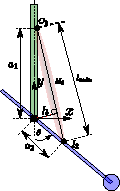
\includegraphics[scale=2.5]{figures/pendulum_moment_arm.pdf}
  \caption[force_length]{Computation of muscle length and moment arm}
  \label{fig:pendulum_muscles_force_length}
\end{figure}

Equation \ref{eq:2} can be extended to the Muscle 2 in similar
way. Thus, the final torque applied by the muscle on to the pendulum
is given by,

\begin{equation}
  \label{eq:3}
  \tau = F \cdot h
\end{equation}

\textbf{NOTE : $\tau$ can also be computed as the cross product of the
  force vector and radial vector. This method is used in the code to
  compute the torques and there by bypassing the moment arm
  computation.}

Where,

\begin{itemize}
\item $\tau$ : Torque [$N \cdot m$]
\item $F$ : Muscle Tendon Force [$N$]
\item $h$ : Muscle Moment Arm [$m$]

\end{itemize}

In this exercise, the following states of the system are integrated
over time,

\begin{equation}
  \label{eq:1}
  X = \begin{bmatrix}
    \theta & \dot{\theta} & A_1 & l_{CE1} & A_2 & l_{CE2}
  \end{bmatrix}
\end{equation}

Where,

\begin{itemize}
\item $\theta$ : Angular position of the pendulum [rad]
\item $\dot{\theta}$ : Angular velocity of the pendulum [rad/s]
\item $A_1$ : Activation of muscle 1 with a range between [0.05, 1].
  0.05 corresponds to base line stimulation and 1 corresponds to
  maximal stimulation.
\item $l_{CE1}$ : Length of contractile element of muscle 1
\item $A_2$ : Activation of muscle 2 with a range between [0.05, 1].
  0.05 corresponds to base line stimulation and 1 corresponds to
  maximal stimulation.
\item $l_{CE2}$ : Length of contractile element of muscle 2
\end{itemize}

To complete this exercise you will make use of the following files,
\fileref{exercise2.py}, \fileref{system\_parameters.py},
\fileref{muscle.py}, \fileref{system.py},
\fileref{pendulum\_system.py}, \fileref{muscle\_system.py},
\fileref{system\_simulation.py} %

\label{sec:questions}

\subsection*{2a. For the given default set of attachment points,
  compute and plot the muscle length and moment arm as a function of
  $\theta$ between $[pi/4, 3pi/4]$ using equations in
  \corr{eqn:\ref{eq:2}} and discuss how it influences the pendulum
  resting position and the torques muscles can apply at different
  joint angles. You are free to implement this code by yourself as it
  does not have any other dependencies.}
\label{sec:2a}


\begin{figure}[H]
  \centering
  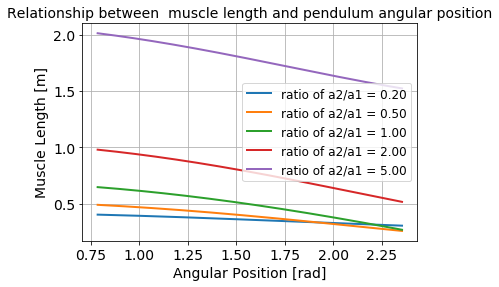
\includegraphics[height=0.3\columnwidth]{Lab6/Report/figures/2a_len.png}
  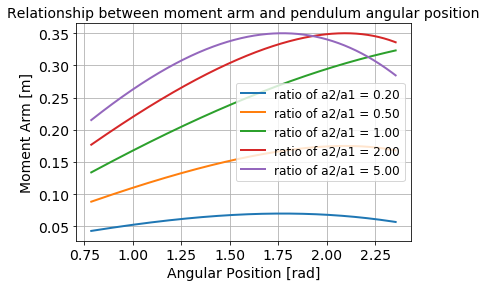
\includegraphics[height=0.3\columnwidth]{Lab6/Report/figures/2a_arm.png}
  \caption{Impact of pendulum angular position on  muscle length and moment arm  }
  \label{2a}
\end{figure}


From equation 2 we can see that this muscle length deceases with increase of $\theta$ if $\theta$ ranges from $\pi/4$ to $3\pi/4$, because in this interval cosine is decreasing. It fits with the observation on upper plot in Figure 4, also we can observe that the decreasing process is slightly nonlinear. The decreasing trend doesn't differ with the different ratios between a1 and a2, but only affects the amplitude. By combining equation 2 and equation 3, we can get h2 as the the single-variable function of $\theta$. This is reflected in the lower plot in Figure 3, in which the moment arm increases until reaching a peak and then decreases.


Since the variable can represent the muscle contraction, we deduce the other muscle length is acting the opposite way. That is, while flexor muscle increases in length, the extensor will shorten. Shorter muscles will has a small angle for muscle in the resting position, and lead to high torques applied.
According to equation 4, he torque is the product of moment arm h and the force developed in the muscle. 
The muscle can be interpret as a flexor. The more the muscle is contracted the higher the force developed in it, and the more the torque it can develop. If the force inside the muscle is fixed, the torque developed by the muscle follows exactly same trend of h shown in Figure 4.




\begin{comment}
\begin{eqnarray}
  L_1 = \sqrt[2]{a_{1}^2 + a_{2}^2 + 2 \cdot a_1 \cdot a_2 \cdot \sin(\theta)} \\
  h_1 = \frac{a_1 \cdot a_2 \cdot \cos(\theta)}{L_1}
\end{eqnarray}
\end{comment}


\subsection*{2b. Using simple activation wave forms (example : sine or
  square waves) applied to muscles (use
  \fileref{system\_simulation.py::add\_muscle\_stimulations} method in
  \fileref{exercise2.py}), try to obtain a limit cycle behavior for
  the pendulum. Use relevant plots to prove the limit cycle behavior.
  Explain and show the activation wave forms you used. Use
  \fileref{pendulum\_system.py::\-PendulumSystem::\-pendulum\_system}
  function to perturb the model.}
\label{sec:2b}

\begin{figure}[H]
  \centering
  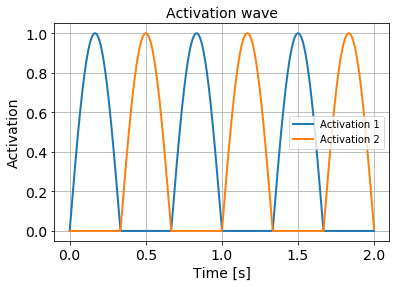
\includegraphics[height=0.3\columnwidth]{Lab6/Report/figures/2b_act.png}
  \caption{Sine activation wave forms }
  \label{2b_act}
\end{figure}

\begin{figure}[H]
  \centering
  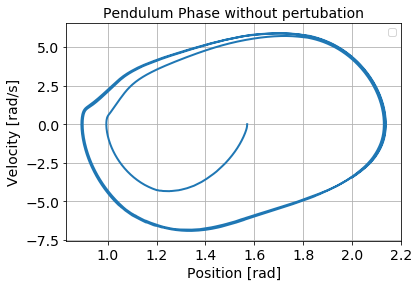
\includegraphics[height=0.3\columnwidth]{Lab6/Report/figures/2b_without.png}
  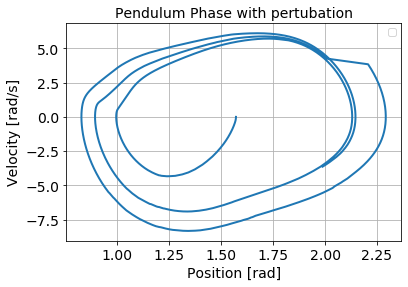
\includegraphics[height=0.3\columnwidth]{Lab6/Report/figures/2b_with.png}
  \caption{Phase plot of pendulum state behavior without and with perturbation }
  \label{2b_phase}
\end{figure}


In this section, we choose sine waves as activation wave. The positive part of the waves are preserved and they have a constant phase shift.
During the simulation, the phase plot shows the system will converge to a closed trajectory when the transient duration is passed (left plot of Figure 6). When the perturbation is applied to the system,it leads to a deviation from the previous trajectory but the system will converge to the closed trajectory as times goes by (right plot of Figure 6). We can deduce that the system has stable limit cycle behaviour, and it's robust to the defaulted perturbation in simulation.
% The phase shift of waves ensures that the two muscles are not activated at the same time but in succession, particularly against each other, but they still fall into a limit cycle through time.


\subsection*{2c. Explore the relationship between stimulation
  frequency with the resulting pendulum's behavior.  Report your
  inferences for a low and high frequency condition.  }
\label{sec:2c}





\begin{figure}[H]
  \centering
  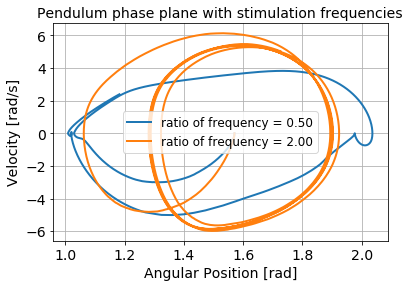
\includegraphics[height=0.3\columnwidth]{Lab6/Report/figures/2c.png}
  \caption{Relationship between stimulation frequency with the resulting pendulum’s behavior}
  \label{2c}
\end{figure}



The behaviours of the system at each frequency converge to a limit cycle after transient phase. With the increase of activation frequency, the amplitude variation of the oscillation of angular position decreases, which fits to the model we discussed in the course. The muscle has less time to contract because in each cycle it is stimulated with less time.
On the other hand, with the increase of activation frequency, the range of variation of the velocity slightly increases, which means the maximal potential velocities will also increase.






\newpage
\section*{Exercise 3 : Neural network driven pendulum model with
  muscles}
\label{sec:neur-netw-driv}

In this exercise, the goal is to drive the above system (Fig
\ref{fig:p_muscles}) with a symmetric four-neuron oscillator
network. The network is based on Brown's half-center model with
fatigue mechanism. Here we use the leaky-integrate and fire neurons
for modelling the network. Figure \ref{fig:p_muscles_neurons} shows
the network structure and the complete system.

\begin{figure}[H]
  \centering
  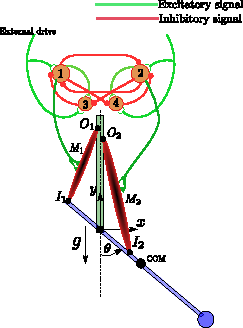
\includegraphics[scale=1.5]{figures/pendulum_muscles_neurons.pdf}
  \caption{Pendulum with Antagonist Hill Muscles Driven Half Center
    Neural Network.}
  \label{fig:p_muscles_neurons}
\end{figure}

Since each leaky-integrate and fire neuron comprises of one first
order differential equation, the states to be integrated now increases
by four(one state per neuron). The states are,


\begin{equation}
  \label{eq:1}
  X = \begin{bmatrix}
    \theta & \dot{\theta} & A_1 & l_{CE1} & A_2 & l_{CE2} & m_1 & m_2 & m_3 & m_4
  \end{bmatrix}
\end{equation}

Where,

\begin{itemize}
\item $m_1$ : Membrane potential of neuron 1
\item $m_2$ : Membrane potential of neuron 2
\item $m_3$ : Membrane potential of neuron 3
\item $m_4$ : Membrane potential of neuron 4
\end{itemize}

To complete this exercise, additionally you will have to use
\fileref{neural\_system.py} and \fileref{exercise3.py}

\subsection*{3a. Find a set of weights and time constants for the
  neural network that produces oscillations to drive the pendulum into
  a limit cycle behavior. Plot the output of the network and the phase
  plot of the pendulum}
\label{sec:4a}

\begin{figure}[H]
  \centering
  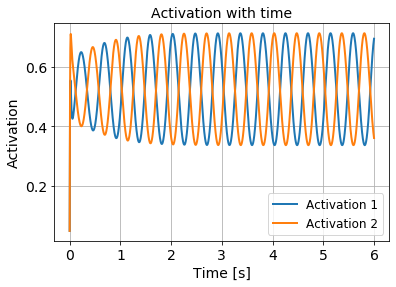
\includegraphics[height=0.3\columnwidth]{Lab6/Report/figures/3a_act.png}
  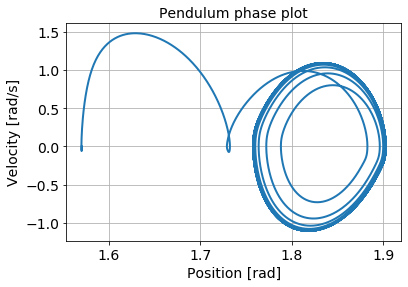
\includegraphics[height=0.3\columnwidth]{Lab6/Report/figures/3a_phase.png}
  \caption{Activation wave forms for muscles (left) and pendulum phase plot (right)}
  \label{3a}
\end{figure}



 In the simulation, We make the simulation time longer than default values (from 2.0s to 6.0s) to observe the system behavior in longer period.
To form an oscillator, the main mechanisms are muscles contraction generation by neuron 1 & 2,
and reciprocal inhibition affected by the other pair.
%According to Figure 8, the output of neurons 1 and 2 are connected with the muscles.
 To be specific, active neuron 1 will stimulate its fatigue neuron, which inhibits neuron 1 and increase the potential of neuron 2 after a short time.
Thus, for this mechanism, there are a pair of inhibiting neurons and they have a larger time constant.



The parameters are selected as follow:
\begin{gather} 
D = 1,\\
\tau=(0.02, 0.02, 0.1, 0.1),\\
b = (3, 3, -3, -3),\\
w=
\left( 
\begin{array}{cccc} 
0 & -5 & 5 & -5 \\ 
-5 & 0 & -5 & 5\\ 
-5 & 0 & 0 & 0 \\ 
0 & -5 & 0 & 0\\
\end{array}
\right) 
\end{gather}
The activation of 2 muscles are balanced due to the shared absolute weights for the neurons, where activation represented by positive weights and inhibition by negative weighs.
It can be observed from Figure 9 that finally the muscles are alternatively activated, the oscillation of the output will become stable and the system converges to a limit cycle.

\subsection*{3b. As seen in the course, apply an external drive to the
  individual neurons and explain how the system is affected. Show
  plots for low [0] and high [1] external drives. To add external
  drive to the network you can use the method \\
  \fileref{system\_simulation.py::add\_external\_inputs\_to\_network}
}
\label{sec:4c}

\begin{figure}[H]
  \centering
  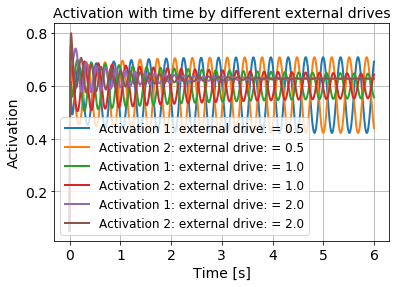
\includegraphics[height=0.3\columnwidth]{Lab6/Report/figures/3b_act.png}
  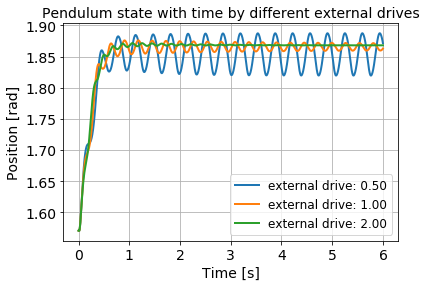
\includegraphics[height=0.3\columnwidth]{Lab6/Report/figures/3b_state.png}
  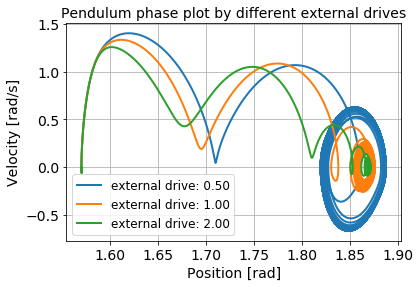
\includegraphics[height=0.3\columnwidth]{Lab6/Report/figures/3b_phase.png}
  \caption{Activation wave forms for muscles (left) and pendulum phase plot (right) with different external drives}
  \label{3b}
\end{figure}



In Figure 10, it can be observed that the system converges to limit cycle and have similar behaviors with the different external drives.
With the increase of external drive, the output amplitude of the 2 activation decreases but their average value (neural position) increases. The position of the pendulum reflects the same trend. 
Actually, there are two types of output, one is the activation (controller for pendulum muscle) and the other is the muscle (system being controlled). The increase of both is aligned with the fact that having a larger input on the system should lead to a larger output in average.
 %As the drive increases, the cycle in phase plot becomes smaller and the average angular position slightly moves towards larger position. 
 The state variance of limit cycle turns to be smaller with larger external drive in our simulation.
 Besides, the oscillation frequency slightly increase with drive from observation.



\subsection*{3c. [Open Question] What are the limitations of the half
  center model in producing alternating patterns to control the
  pendulum? What would be the effect of sensory feedback on this
  model? (No plots required)}
\label{sec:4d}

%(不确定,有待验证)
As we can see on Figure 10, we infer that with the increase of external drive the muscle activation (force) and the frequency increase. If we focus on the lamprey using this model and put it into a pool. If the lamprey needs to overcome the backflow (disturbance) which block the forward motion of lamprey, more force has to be built, meaning that the external drive has to be increased, leading to smaller steps as well as fast movement. However, the smaller step cycle may course problem in the simple model without sensory feedback due to the limitation of coupling.
With sensory feedback, the lamprey can easily handle this problem through local pressure feedback, thus leading to better state stabilization and behavior adjustment by outside environment. 
Besides, sensory feedback can also provide more complexity of system behavior. For example, if the model is implemented on the leg muscle, more real and reasonable gait can be realized. Combined with muscle feedback unit like spindles and golgi tendon organs, stumbling correction and leg extension can be implemented for alternative gait behaviors.
Another benefit of sensory feedback is that it can provide information upon which the neural network can learn and train its parameter through advanced techniques like reinforcement learning.
Thus the feedback can provide strong robustness and behavior diversity.



\newpage
\section*{Appendix I : Hill muscle model equations}
\label{sec:hill-model-equations}
\begin{table}[H]
  \centering
  \begin{tabular}{c|c|p{7cm}}
    \textbf{Name}& \textbf{Equation}& \textbf{Comment} \\ \hline
    $F_{mtu}$ & $F_{m} = F_{se} = F_{ce}+F_{pe}-F_{be}$ & Force of generated by the MTU \\[0.7cm]
    $F_{se}$ & $
               F_{se}=
               \begin{cases}
                 F_{max} \cdot (\frac{\varepsilon}{\varepsilon_{ref}})^2,& \text{if } \varepsilon > 0 \\
                 0, & \text{otherwise}
               \end{cases}
                      $  & Force generated by the tendon \\[0.7cm]
    $F_{pe}$ & $
               F_{pe}=
               \begin{cases}
                 F_{max} \cdot (\frac{l_{ce}-l_{opt}}{l_{opt}w})^2\cdot f_{v}(v_{ce}),& \text{if } l_{ce} > l_{opt} \\
                 0, & \text{otherwise}
               \end{cases}
                      $
                                    & Force of the parallel element preventing muscle overextension \\[0.7cm]
    $F_{be}$ & $
               F_{be}=
               \begin{cases}
                 F_{max} \cdot (\frac{l_{opt}-w-l_{ce}}{l_{opt}w/2})^2,& \text{if } l_{ce} \leq l_{opt}\cdot(1 - w) \\
                 0, & \text{otherwise}
               \end{cases}
                      $
                                    & Force of the parallel element preventing muscle to collapse
    \\[0.7cm]

    $F_{ce}$ & $F_{ce} = A \cdot F_{max} \cdot f_l(l_{ce}) \cdot f_v(v_{ce})$ & Force generated by the muscle (ce) \\ [0.7cm]

    $A$ & $\frac{dA}{dt} = \tau \cdot (S(t) - A)$ & Muscle activation is equal to the integral of the input signal I(t). Biologically, the input signal can be viewed as the normalized frequency of neuronal spike that reaches the muscle (i.e. restricted to the [0.05; 1] interval). The activation is thus also limited to this interval. \\[0.7cm]

    $f_l({l_{ce}})$ & $f_l({l_{ce}}) = exp(c|\frac{l_{ce}-l_{opt}}{l_{opt}w}|^3)$ & Muscle force - muscle length relationship function (function of the
                                                                                    muscle length (lce) \\[0.7cm]

    $f_{v}(v_{ce})$ & $f_{v}(v_{ce}) = \begin{cases}
      \frac{v_{max}-v_{ce}}{v_{max}+k \cdot v_{max}},& \text{if } v_{ce} < 0 \\
      N + (N - 1)\frac{v_{max}-v_{ce}}{7.56 \cdot K \cdot v_{ce} - v_{max}}, & \text{otherwise}
    \end{cases}$ & Muscle force - muscle velocity relationship function (function of the muscle velocity (vce ) \\[0.7cm]

    $v_{ce}(f_{v})$ &  $v_{ce}(f_{v}) = \begin{cases}
      v_{max} \cdot \frac{1 -f_v }{1 + f_v \cdot K},& \text{if } f_{v} < 1.0 \\
      v_{max} \cdot \frac{f_v - 1}{7.56 \cdot K \cdot (f_v - N) + 1 - N}, & \text{otherwise}
    \end{cases}$ & Inverse of the muscle force - velocity
                   function. This function is used for the resolution of the muscles equations. \\[0.7cm]
    $l_{ce}$ & $\int v_{ce} \cdot dt$ & Muscle (ce) length \\[0.7cm]
    $l_{se}$ & $l_{se} = l_{mtu} - l_{ce}$ & Tendon (se) length \\[0.7cm]
    $l_{mtu}$ & $l_{mtu} = l_{opt} + l_{slack} + \delta l_{mtu}$ & MTU
                                                                   length
  \end{tabular}
  \label{tab:hill-eqn}
\end{table}

\end{document}
